\documentclass{beamer}
\graphicspath{{../graphics/}}
\usepackage{listings}
\usepackage{ulem}
\usepackage{subcaption}
\captionsetup{compatibility=false}
\usepackage[linesnumbered]{algorithm2e}
\usepackage{multicol}

\newcommand{\linespace}{\vspace{1em}}

\mode<presentation>
{
  \usetheme{Darmstadt}
  \setbeamertemplate{footline}[frame number]
  \setbeamertemplate{navigation symbols}{}
  \setbeamercovered{transparent}
}

\AtBeginSection[]
{
   \begin{frame}
        \frametitle{Indhold}
        \tableofcontents[sectionstyle=show/hide,subsectionstyle=show/show/hide]
   \end{frame}
}

\usepackage[danish]{babel}
\usepackage[T1]{fontenc}

\usepackage[utf8]{inputenc}

\usepackage{times}

\usepackage{tikz}
\usepackage{multirow}

\title[Stemmespillet]{Stemmespillet}

\subtitle{SW613F14}

\author[SW613F14]{
Mikael Elkiær Christensen \\\and
Mikkel Sandø Larsen \\\and
Stefan Marstrand Getreuer Micheelsen \\\and
Bruno Thalmann
}

\institute[Aalborg Universitet]
{
  Software\\
  Aalborg Universitet}

\date[CFP 2003]{16. juni 2014}

\begin{document}

%--------------------------------------------------
%     INTRODUKTION
%--------------------------------------------------

\begin{frame}
  \titlepage
\end{frame}

\begin{frame}
    \frametitle{Indhold}
    \tableofcontents[sectionstyle=show/show,subsectionstyle=hide/hide/hide]
\end{frame}

\section{Multiprojekt}

% % %
% GIRAF
% % %
\subsection{GIRAF}

\begin{frame}
\frametitle{Filosofi}

\begin{itemize}
\item \textit{Graphical Interface and Resources for Autistic Folk} (GIRAF)
\item Ét samlet værktøj med mange funktioner
\item Skal gøre livet nemmere for personer med autisme, samt deres forældre/pædagoger
\item Skal fungere som institutioners eneste værktøj, derved også administration
\end{itemize}

\end{frame}

\begin{frame}
\frametitle{Opbygning}

\begin{itemize}
\item Launcher (GIRAF)
\begin{itemize}
\item 2 tilstande
\begin{itemize}
\item Citizen, Guardian
\end{itemize}
\item Tilpasning til den enkelte profil
\begin{itemize}
\item Valg af applikationer
\item Indstillinger for applikationer
\end{itemize}
\end{itemize}
\item Applikationer
\begin{itemize}
\item Praktiske
\begin{itemize}
\item PictoOplæser, Sekvens, Timer
\end{itemize}
\item Administrative
\begin{itemize}
\item Administration (findes også som web-app)
\end{itemize}
\item Læring
\begin{itemize}
\item Stemmespillet, Kategorispillet
\end{itemize}
\end{itemize}
\end{itemize}

\end{frame}

\begin{frame}
\frametitle{Kunden}

\begin{itemize}
\item 6 kunder
\begin{itemize}
\item 4 pædagoger i Specialbørnehaven Birken
\item 1 lærer på Egebakken
\item 1 talepædagog, tilknyttet Aalborg Kommune
\end{itemize}
\end{itemize}

\end{frame}

% % %
% ORGANISATION
% % %
\subsection{Organisation}

\begin{frame}
\frametitle{Opbygning}

\begin{itemize}
\item Scrum of scrums
\begin{itemize}
\item 16 grupper
\item 1 statusgruppe
\item 4 sprints
\end{itemize}
\end{itemize}

\centering\includegraphics[height=.5\textheight]{pgraphics/scrum-of-scrums}

\end{frame}

\begin{frame}
\frametitle{Møder}

\begin{itemize}
\item Ugentlige statusmøder
\begin{itemize}
\item Status
\item Problemer
\item Dagsorden
\end{itemize}
\item Fælles sprint review
\item Fælles sprint planning
\end{itemize}

\end{frame}

\begin{frame}
\frametitle{Samarbejde}

\begin{itemize}
\item Fælles komponenter
\begin{itemize}
\item Database
\begin{itemize}
\item RemoteDb
\item LocalDb
\item OasisLib
\end{itemize}
\item giraf-components
\item Mindre dele
\begin{itemize}
\item Sekvens og Livshistorier
\end{itemize}
\end{itemize}
\item Værktøjer
\begin{itemize}
\item Redmine
\item Git
\item Jenkins
\end{itemize}
\item Specialister
\end{itemize}
%FORDELE ULEMPER

\end{frame}

% % %
% CARS
% % %
\subsection{Cars}

\begin{frame}
\frametitle{Filosofi}

\begin{itemize}
\item Formål
\begin{itemize}
\item Udvikling af stemmen
\item Styring af stemmen
\item Stemme ud fra kontekst
\end{itemize}
\item Brug
\begin{itemize}
\item Pædagog sidder med borger og spiller spillet
\item Kan i situation refereres til spil
\item Kan under spil refereres til situation
\end{itemize}
\end{itemize}

\end{frame}

\begin{frame}
\frametitle{Anekdoter}

\begin{itemize}
\item Borger hænger i træ og kan ikke komme ned, hvisker efter hjælp
\item Borger sidder ved middagsbordet, råber efter saltet
\end{itemize}

\end{frame}

\begin{frame}
\frametitle{Udvikling}

\begin{columns}

\begin{column}{.48\textwidth}
\begin{itemize}
\item Sprint 1
\begin{itemize}
\item Gamle krav
\item Styring via volume
\item Refaktorering (framework)
\end{itemize}
\item Sprint 2
\begin{itemize}
\item Begyndende implementering
\item Første interview
\item Nye krav
\end{itemize}
\end{itemize}
\end{column}

\begin{column}{.48\textwidth}
\begin{itemize}
\item Sprint 3
\begin{itemize}
\item Implementering af krav
\item Brug af database/GUI
\item Forbedring af styring
\end{itemize}
\item Sprint 4
\begin{itemize}
\item Vigtigste interview
\item Nye krav
\item Implementering af nye krav
\end{itemize}
\end{itemize}
\end{column}

\end{columns}

\end{frame}

\begin{frame}
\frametitle{Fremgangsmåde}

\begin{columns}

\begin{column}{.48\textwidth}
\begin{itemize}
\item Scrum
\item Morgenmøde
\item Scrumboard
\begin{itemize}
\item Stories
\item Tasks
\item Planning poker
\end{itemize}
\item Tasks ud fra krav
\end{itemize}
\end{column}

\begin{column}{.48\textwidth}
\includegraphics[width=\textwidth]{pgraphics/scrumboard}
\end{column}

\end{columns}

\end{frame}
\section{Kundekontakt}

\subsection{Interviews}

\begin{frame}{Udførte Interviews}
To interviews blev udført 

\begin{itemize}
\item 4. April, 2. sprint - to pædagoger fra Birken \\ Præcisering af gamle krav
\item 8. Maj, 4. sprint - talepædagog \\Feedback fra oprindelig kontaktperson på Cars 
\end{itemize}

\end{frame}

\begin{frame}{Metode}
\begin{itemize}
\item Semistruktureret interview 
\item Åbne spørgsmål 
\begin{itemize}
\item ideer
\item feedback
\end{itemize}
\item Sætter en samtale igang om tilstanden af applikationen
\end{itemize}
\end{frame}

\begin{frame}{Resultat}
\begin{itemize}
\item Præcisering af krav
\item Nye krav
\item Feedback på produktet
\end{itemize}
\end{frame}

\begin{frame}{Problemstillinger}
\begin{itemize}
\item Interview timing
\begin{itemize}
\item Forkert email
\item Det vigtigste interview kom meget sent
\end{itemize}
\item Kunder skifter mening
\begin{itemize}
\item Forskellige kunder har forskellige meninger
\item Ændrer mening når implementation vises
\item Forskellig opfattelse af krav
\end{itemize}
\end{itemize}
\begin{center}
\includegraphics[width=0.8\textwidth]{pgraphics/whatthecostumerwanted}
\end{center}
\end{frame}

\subsection{Kravstyring}

\begin{frame}{Opdatering af krav}
\begin{itemize}
\item Baseret på udførte interviews
\item Userstories, tasks
\end{itemize}

\begin{center}
\includegraphics[width = 0.7\textwidth]{pgraphics/tasks}
\end{center}
\end{frame}

\begin{frame}{Fælles krav}
Der blev vedtaget krav fælles for alle projekter
\begin{itemize}
\item Uformelle 
\item Svære at holde styr på
\end{itemize}

Eksempler:
\begin{itemize}
\item GUI
\item Navne på projekter
\item Profilvælger
\end{itemize}
\end{frame}

\begin{frame}{Eksempel}
Fra original Cars rapport
\begin{itemize}
\item \textit{It must be possible for the user to change the difficulty of the game}
\end{itemize}

Efter første interview
\begin{itemize}
\item \textit{Speed is alterable. The speed level is represented as a digit between 0 and 10.}
\item \textit{The placement and number of obstacles is alterable}
%\item The placement of obstacles should be in such a way, that it is possible to adapt it to both citizen with tendency to speaking too loud as well as those speaking too low.
\item\textit{ It should be possible, in settings, to switch\\ between avoiding objects and picking objects up.}
\end{itemize}
\end{frame}

\section{Design}


\subsection{Framework}
\begin{frame}
\frametitle{Brug af framework}
\begin{itemize}
\item Abstraherer væk fra Android platformen
\item Opbygget omkring brug af forskellige \textit{''screens''}
\item Spillet er indeholdt i en \textit{''activity''}
\item Til grafik og lyd er der en klasse til hver der eksponerer basale metoder
\item \textit{''Deltatime''} er den tid der går mellem hver frame
\end{itemize}
\end{frame}


\subsection{Mål med spillet}
\begin{frame}
\frametitle{Gamle Cars}
Undgå forskellige forhindringer og køre i den garage som har den samme farve som bilen
\begin{figure}
\includegraphics[width=130px]{sprint1/cars_screenshot}
\end{figure}
\end{frame}

\begin{frame}
\frametitle{Nuværende Cars}
\begin{itemize}
\item Krav sprint 2: \textit{The goal of the game is to reach a garage}
\item Krav sprint 4: \textit{The goal of the game is to reach the finishing line
after successfully collecting all items or avoiding
all items (two different game modes)}
\end{itemize}
\begin{figure}
\begin{subfigure}[b]{0.4\textwidth}
\includegraphics[width=125px]{sprint2/sound_gauge}
\caption{Sprint 2}
\end{subfigure}
~
\begin{subfigure}[b]{0.4\textwidth}
\includegraphics[width=125px]{sprint4/game}
\caption{Sprint 4}
\end{subfigure}
\end{figure}
\end{frame}


\subsection{Kontrol af bil}
\begin{frame}
\frametitle{Det gamle Cars}
\begin{itemize}
\item Kontrol af bilen var baseret på frekvens
\item Det var svært at styre, hvis ikke umuligt
\end{itemize}
\begin{figure}[h]
\centering
\begin{subfigure}[t]{.45\textwidth}
\includegraphics[width=\textwidth]{sprint1/spectrum_tonegenerator}
\caption{Frequency spectrum for a 440 Hz generated tone}
\end{subfigure}
\begin{subfigure}[t]{.45\textwidth}
\includegraphics[width=\textwidth]{sprint1/spectrum_highpitchvoice}
\caption{Frequency spectrum for human voice input (in an attempt to reach 1200Hz)}
\end{subfigure}
\end{figure}
\end{frame}

\begin{frame}
\frametitle{Sprint 2}
\begin{itemize}
\item Skiftet fra frekvens til volumen
\item Krav: \textit{The car is controlled in such a way,
that the vertical position of the car is relative
to the current loudness of the player's voice.}
\end{itemize}
\begin{figure}
\centering
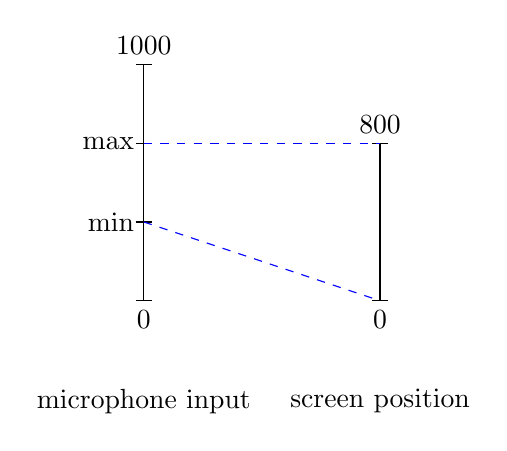
\begin{tikzpicture}
%vertical scales
\draw (0,0) -- (0,3); 
\draw (3,0) -- (3,2);

\node [below] at (0,-1){microphone input};
\node [below] at (3,-1){screen position};

%  endpoints with labels
\draw (-0.1,0) -- (0.1,0); 
\node [below] at (0,0){0};

\draw (-0.1,3) -- (0.1,3);
\node [above] at (0,3){1000};

\draw (2.9,0) -- (3.1,0); 
\node [below] at (3,0){0};

\draw (2.9,2) -- (3.1,2);
\node [above] at (3,2){800};

%min and max labels 
\draw (-0.1,1) -- (0.1,1);
\node [left] at (0,1){min};

\draw (-0.1,2) -- (0.1,2);
\node [left] at (0,2){max};

% mapping lines
\draw [dashed, blue](0,2) -- (3,2);
\draw [dashed, blue](0,1) -- (3,0);
\end{tikzpicture}
\end{figure}
\end{frame}

\begin{frame}
\frametitle{Sprint 3}
\begin{itemize}
\item Stabilisering af bilen
\item Forskellige afprøvede metoder:
\begin{itemize}
\item Gennemsnit
\item Acceleration og deceleration (valgt)
\end{itemize}
\end{itemize}
\end{frame}


\subsection{Kalibrering}
\begin{frame}
\frametitle{Kalibrering af mikrofonen}
\begin{itemize}
\item Krav: \textit{It must be possible to calibrate the microphone}
\item Kalibreringen sætter en max og en min værdi
\item Projektets problembarn
\item Den grafiske fremstilling i indstillinger var meget udfordrende
\end{itemize}
\end{frame}

\begin{frame}
\frametitle{Visuel udvikling}
\begin{figure}
\begin{subfigure}[b]{0.4\textwidth}
\includegraphics[width=130px]{sprint2/settings}
\caption{The settings activity from sprint 2}
\end{subfigure}
~
\begin{subfigure}[b]{0.4\textwidth}
\includegraphics[width=130px]{sprint4/settings_s4}
\caption{The settings activity from sprint 4}
\end{subfigure}
\end{figure}
\end{frame}


\subsection{Map editor}
\begin{frame}
\frametitle{Sprint 2}
\begin{itemize}
\item Krav: \textit{The placement and number of obstacles is alterable.}
\item Krav: \textit{The placement of obstacles should be
in such a way,
that it is possible to adapt it to both citizen
with tendency to speaking too loud
as well as those speaking too low.}
\end{itemize}
\begin{figure}[h]
\includegraphics[width=0.5\linewidth]{sprint2/map_editor}
\end{figure}
\end{frame}

\begin{frame}
\frametitle{Sprint 4}
\begin{figure}[h]
\includegraphics[width=\linewidth]{sprint4/mapeditor}
\end{figure}
\end{frame}

\subsection{Barometre}
\begin{frame}
\frametitle{Barometre fra institutionen}
\begin{figure}[h]
	\centering
        \begin{subfigure}[b]{0.4\textwidth}
                \includegraphics[width=\textwidth]{sprint2/sound}
                \caption{Lydbarometer}
        \end{subfigure}%
        ~
        \begin{subfigure}[b]{0.4\textwidth}
                \includegraphics[width=\textwidth]{sprint2/speed}
                \caption{Hastighedsbarometer}
        \end{subfigure}
\end{figure}
\end{frame}

\begin{frame}
\frametitle{Lydebarometer}
\begin{itemize}
\item Tal mellem 0 og 10 på bil, forhindringer og stjerner
\item Mulighed for at pause spillet og se hvor man er henne på barometret
\end{itemize}
\begin{figure}
\includegraphics[width=200px]{sprint2/pause}
\end{figure}
\end{frame}

\begin{frame}
\frametitle{Hastighedsbarometer}
\begin{itemize}
\item Vælge hastighed ud fra et barometer
\end{itemize}
\begin{figure}
\includegraphics[width=200px]{sprint4/settings_s4}
\end{figure}
\end{frame}
\section{Opsummering}
\subsection{}
\begin{frame}
\frametitle{Demonstration}
\begin{center}
\includegraphics[width=2.5cm]{barn_tablet}
\end{center}
\end{frame}
\begin{frame}
\frametitle{Kalibrering}
\end{frame}

\begin{frame}
\frametitle{Forskellige skærmstørrelser}
\end{frame}
%Skal der inkluderes noget fra reflections?

\end{document}